\documentclass[11pt]{article}

% Packages
\usepackage{graphicx}   % for pictures
\usepackage{amsthm}     % for math
\usepackage{amsmath, mathtools}    %   more math
\usepackage{amsfonts}   %   more math
\usepackage{physics}    % more symbols
\usepackage{circuitikz} % for circuit diagrams
\usepackage{amssymb}    % math symbols
\usepackage{siunitx}    % units
\usepackage{mathrsfs}   % fancy text
\usepackage{color}      % colored letters for notes and reminders
\usepackage{float}      % for image location

%The amsthm package lets you format different types of mathematical ideas nicely. You use it by defining "\newtheorem"s as below:
\newtheorem{problem}{Problem}
\newtheorem{theorem}{Theorem}
\newtheorem*{proposition}{Proposition}
\newtheorem{lemma}[theorem]{Lemma}
\newtheorem{corollary}[theorem]{Corollary}
\theoremstyle{definition}
\newtheorem{defn}[theorem]{Definition}

% Magins

\setlength{\voffset}{0.1in}
\setlength{\paperwidth}{8.5in}
\setlength{\paperheight}{11in}
\setlength{\headheight}{14pt}
\setlength{\headsep}{0.5in}
\setlength{\textheight}{11in}
\setlength{\textheight}{8in}
\setlength{\topmargin}{-0.25in}
\setlength{\textwidth}{7in}
\setlength{\topskip}{0in}
\setlength{\oddsidemargin}{-0.25in}
\setlength{\evensidemargin}{-0.25in}

% For images in this document:
\graphicspath{ {images/} }

% User Defined Commands
\newcommand{\nder}[2]{\frac{d^{#1} #2}{d t^{#1}}}   % The nth derivative wrt t: {n}{x(t)}
\newcommand{\der}[1]{\frac{d #1}{d t}}              % Derivative wrt t: {x(t)}
\newcommand{\infint}{\int_{-\infty}^{\infty}}       % Integral from - infinity to + infinity
\newcommand{\infsum}[1]{\sum_{#1 = -\infty}^{\infty}}% Sum of a variable from - to + infinity
\newcommand{\para}[1]{\left( #1 \right)}            % Instead of writing parenthesis all the time

% User Command for Wider Matrices
\makeatletter
\renewcommand*\env@matrix[1][\arraystretch]{%
  \edef\arraystretch{#1}%
  \hskip -\arraycolsep
  \let\@ifnextchar\new@ifnextchar
  \array{*\c@MaxMatrixCols c}}
\makeatother


% Heading:
\usepackage{fancyhdr}
\pagestyle{fancy}
\lhead{Nicholas Pham}
\chead{ES 155}          %   Change the Class!!
\rhead{Homework 6}   %   Change the Problem Set Number!!


% ----- BEGIN DOCUMENT-----
\begin{document}

\textbf{\huge{ES 155 Homework 6}}    %   Change the Class and Problem Set Number!!
\normalsize

\begin{enumerate}
    \item % Problem 1
    \begin{figure}[H]
        \centering
        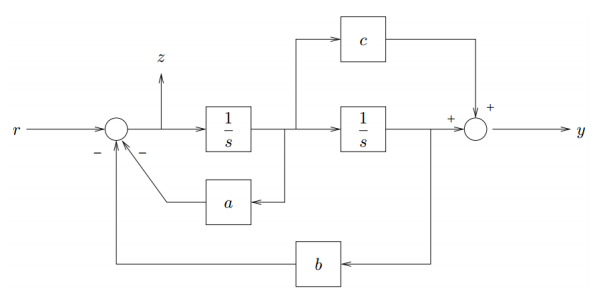
\includegraphics[width = 0.8\textwidth]{ES155P6_1block.png}
        \caption{System Block Diagram}
        \label{fig:problem1block}
    \end{figure}
    \begin{enumerate}
        \item % 1.a
        To compute the transfer function for the block diagram in Figure \ref{fig:problem1block}, first add some additional labels.  Let $Z$ be the output of the first summing node on the left, $A$ be the output of the first integrator, and $B$ be the output of the second integrator.  This gives

        \begin{align*}
            Z(s) &= R(s) - aA(s) - bB(s) \\
            Z(s) &= sA(s) \\
            A(s) &= sB(s) \\
            Y(s) &= B(s) + cA(s)
        \end{align*}

        With four equations and four unknowns, we can plug in to solve for $Y(s) = H_{yr}(s) R(s)$

        \begin{align*}
            Y(s) &= B(s) + cA(s) = B(s) + csB(s) \\
            B(s) &= \frac{Y(s)}{1 + cs} \\
            Z(s) &= sA(s) = R(s) - aA(s) - bB(s) \\
            s^2 B(s) &= R(s) - asB(s) - bB(s) \\
            R(s) &= \left( s^2 + asB(s) + bB(s) \right)B(s) \\
            \frac{Y(s)}{1 + cs} &= \frac{1}{s^2 + as + b}R(s) \\
            H_{ry} &= \frac{1 + cs}{s^2 + as + b}
        \end{align*}
        \item % 1.b
        The state space system

        \begin{align*}
            \dot{x} &= Ax + Bu = \frac{d}{dt} \begin{bmatrix} x_1 \\ x_2 \end{bmatrix} = \begin{bmatrix} 0 & 1 \\ -a_2 & -a_1 \end{bmatrix} \begin{bmatrix} x_1 \\ x_2 \end{bmatrix} + \begin{bmatrix} 0 \\ 1 \end{bmatrix} r \\
            y &= Cx + Du = \begin{bmatrix} b_2 & b_1 \end{bmatrix} \begin{bmatrix} x_1 \\ x_2 \end{bmatrix} + d \cdot r
        \end{align*}

        can be written 

        \begin{align*}
            \dot{x_2} &= -a_2 x_1 - a_1 x_2 + r \\
            &= -a_2 x_1 - a_1 \dot{x_1} + r \\
            y &= b_2 x_1 +  b_1 x_2 + dr \\
            &= b_2 x_1  + b_1 \dot{x_1} + dr \\
        \end{align*}

        In the Laplace domain

        \begin{align*}
            s^2 X_1 &= -a_2 X_1 - a_1 s X_1 + R \\
            X_1 &= \frac{1}{s^2 + a_1 s + a_2} R \\
            Y &= b_2 X_1 + b_1sX_1 + d \cdot R \\
            &= (b_2 + b_1s) \frac{1}{s^2 + a_1 s + a_2} R + d \cdot R \\
            &= \left( \frac{b_2 + b_1 s}{s^2 + a_1s + a_2} + d \right) R
        \end{align*}

        which is has the same transfer function as part a) for $a_1 = a, a_2 =b, b_1 = c, b_2 = 1, d = 0$.

        \item % 1.c
        The transfer function $H_{zr}$ can also be computed.

        \begin{align*}
            Z &= R + aA - bB = R - a \frac{1}{s}Z - b \frac{1}{s^2}Z \\
            Z\left( 1 + \frac{a}{s} + \frac{b}{s^2} \right) &= R \\
            Z &= \frac{s^2}{s^2 + sa + b} R \\
            H_{rz} &= \frac{s^2}{s^2 + sa + b}
        \end{align*}
    \end{enumerate}

     \item % Problem 2
     A simple cruise control system has the equations of motion

     \begin{align*}
        m \dot{v} &= -cv + b \tau + F_{\text{hill}} \\
        \dot{\tau} &= a( -\tau + Tu)
     \end{align*}

    \begin{enumerate}
        \item % 2.a
        With controller $u = k_p e$ where $e = r - v$, the system can be written as a block diagram of each of the components.  First compute their transfer functions need to be computed.  $H_U = k_p$ is easy.  The engine torque transfer function is 

        \begin{align*}
            s\tau &= -a\tau + aTU \\
            \tau &= \frac{aT}{s + a}U \\
            H_\tau &= \frac{aT}{s + a}
        \end{align*}

        Finally, the velocity in the $s$-domain (where $F_\text{hill} \text{ is } d$) can be written 

        \begin{align*}
            msV(s) &= -cV(s) + b\tau(s) + D(s) \\
            V(s) &= \frac{b\tau(s) + D(s)}{ms + c}
        \end{align*}

        Because it takes two inputs ($\tau(s)$ and $D(s)$), this block is broken up in the block diagram, shown in Figure 

        \begin{figure}
            \centering
            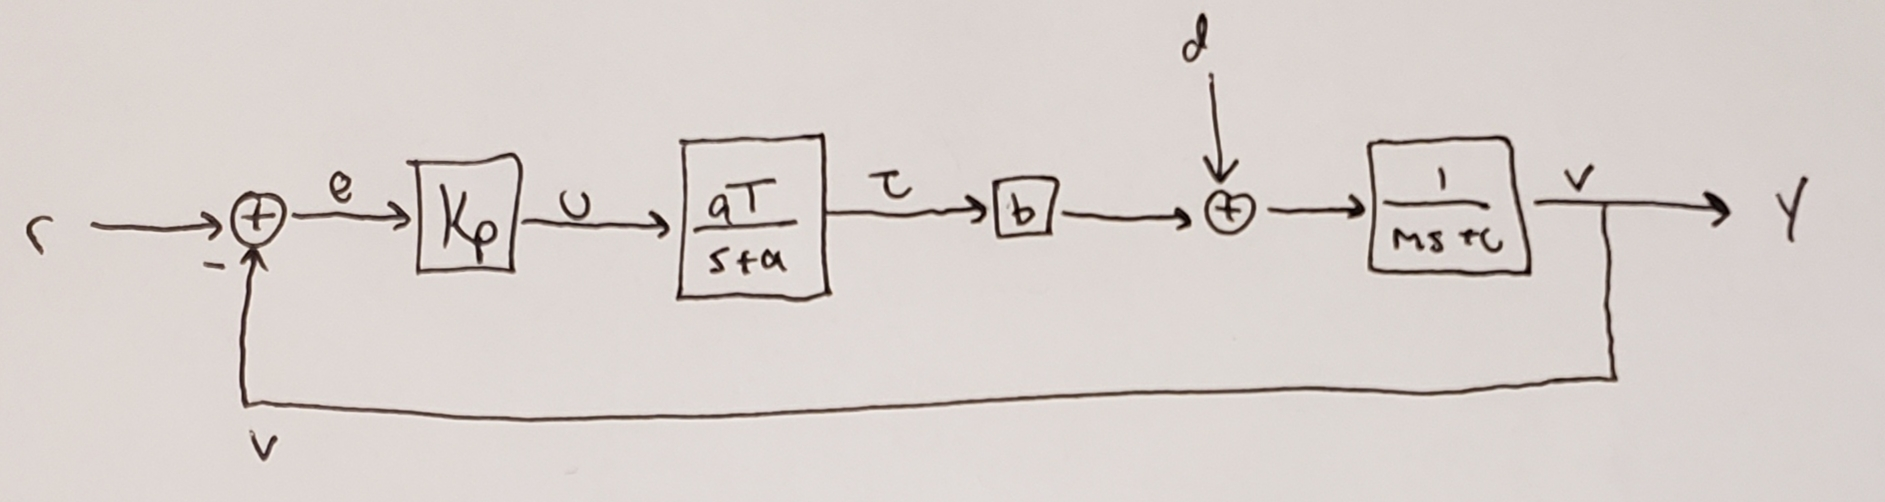
\includegraphics[width = 0.8\textwidth]{blocka.jpg}
            \caption{Block Diagram of Simple Cruise Control System}
            \label{fig:p_control}
        \end{figure}

        \item % 2.b
        The transfer function of the entire system can be broken down as several individual blocks, as shown in part (a).  Because the transfer function of two blocks connected in series is the product of their indivdual transfer functions, the overall transfer function can be computed in MATLAB using this technique along with the $\mathtt{feedback}$ function.  

        See MATLAB for the system simulation, computed via the transfer function, and the step response and bode plots of the system with $k_p = 0.01$ and $k_p = 0.1$, which is shown in Figure \ref{fig:plots_b}.

        \begin{figure}
            \centering
            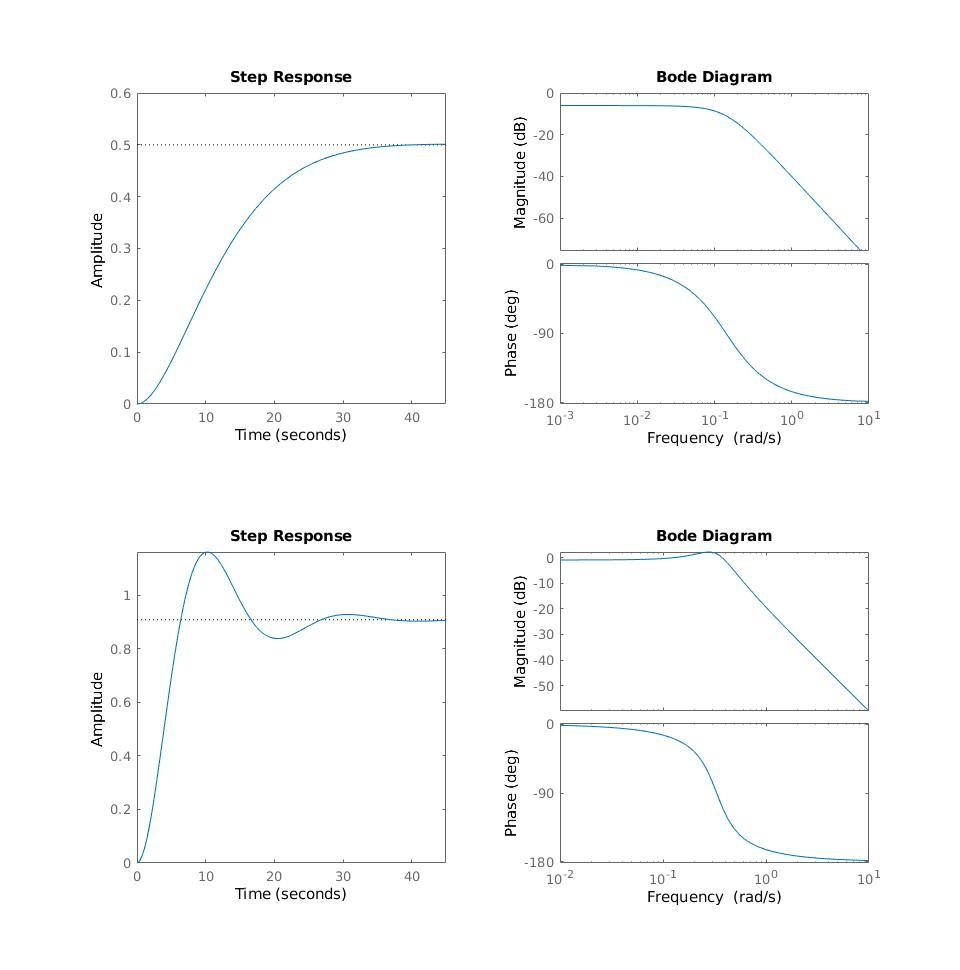
\includegraphics[width = 0.8\textwidth]{155P6_2b.jpg}
            \caption{System characterization plots.  On top is the step response and bode plot when $k_p = 0.01$, while the bottom shows the step response and bode plot for $k_p = 0.1$}
            \label{fig:plots_b}
        \end{figure}

        As can be seen in the plot, the step response of the system with $k_p = 0.01$ has little oscillation, but has a rather large long term error, as it asymptotically reach 0.5 instead of the desired value of 1.  Increasing $k_p$ to 0.1 increases the oscillation and overshoot, but the long term error is decreased.  The magnitude Bode plot now shows a peak.  

        \item % 2.c
        With a proportional and integral control law $u = k_p e + k_i x_c$ where $\frac{d}{dt}x_c = e = r - v$.  This means that the transfer function for the control block is 

        \begin{align*}
            u &= k_p e + k_i \int e \\
            U(s) &= k_p E(s) + k_i \frac{1}{s}E(s) \\
            H_U &= k_p + k_i \frac{1}{s}
        \end{align*}

        Again, the overall transfer function is computed in MATLAB.  Figure \ref{fig:pi_control} shows a block diagram of the system with this more complex control law, assuming $d = 0$.

        \begin{figure}
            \centering
            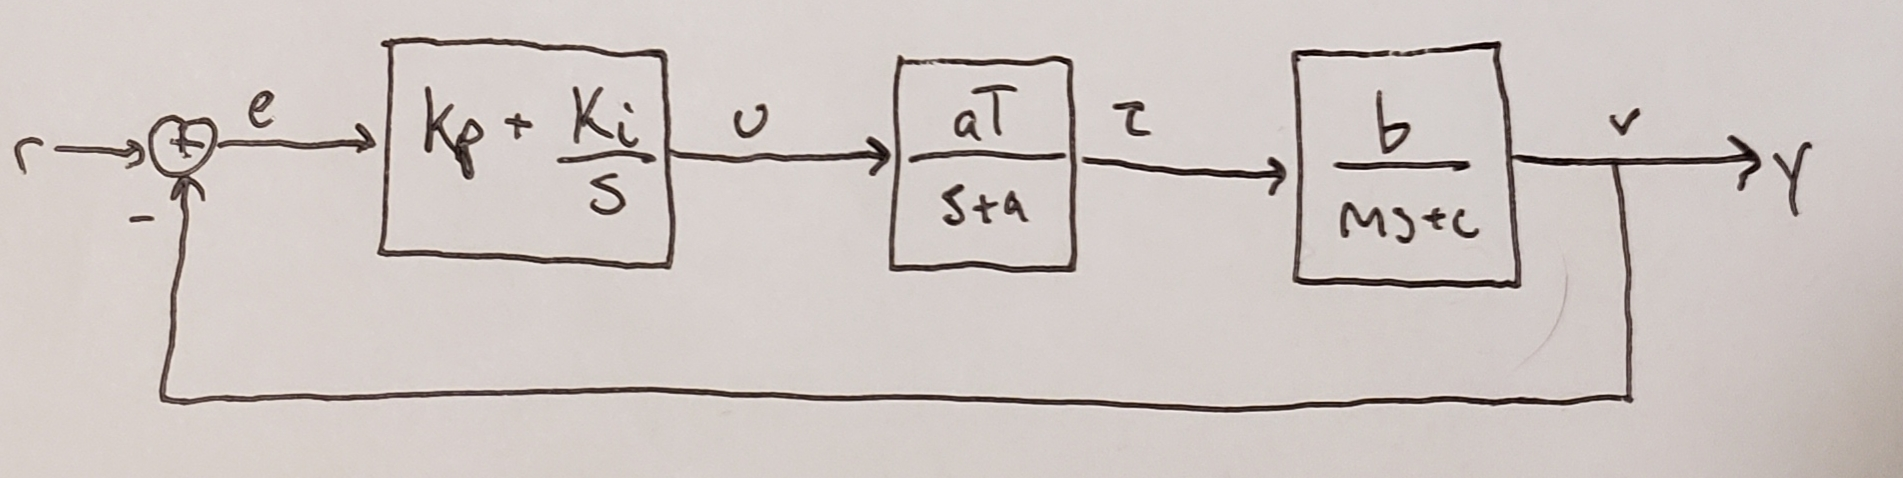
\includegraphics[width = 0.7\textwidth]{blockc.jpg}
            \caption{Block diagram of the system with the more complex control law}
            \label{fig:pi_control}
        \end{figure}

        \item % 2.d
        See the MATLAB code for the computation and plotting of the step and frequency response.  Figure \ref{fig:pi_plots} shows these plots.  The magnitude Bode plot now shows a strong peak, and the step response is highly oscillitory.  Though the overshoot is now almost 100\%, the long term error appears to go to zero.  The addition of this integral control trades an increase in overshoot and oscillation for a reduction in long term error.

        \begin{figure}
            \centering
            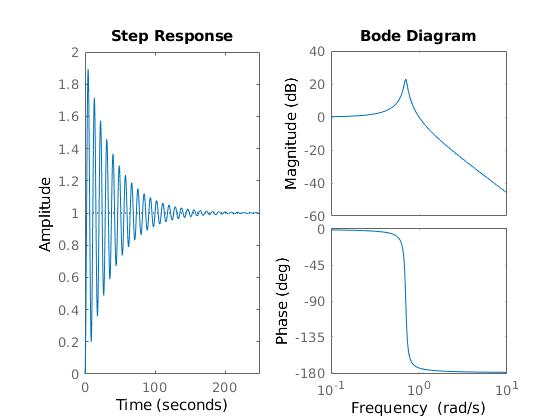
\includegraphics[width = 0.8\textwidth]{155P6_2d.jpg}
            \caption{Step response and Bode plot for the systemw ith proportional and integral control law.}
            \label{fig:pi_plots}
        \end{figure}

    \end{enumerate}
\end{enumerate}
\end{document}


